\documentclass[10pt,a4paper]{article}

%double si on veut une version prof et une version élève. simple si on veut une seule version.
\newcommand{\buildmode}{double}

\InputIfFileExists{version.tex}{}{}
% Version (définie par le script)
\providecommand{\version}{eleve}

\usepackage{feuilleactivite}

%%%à modifier à chaque fois

\renewcommand{\niveau}{2nde}
\renewcommand{\chapitre}{Distance entre deux nombres, valeur absolue}
\renewcommand{\numchap}{0.3}
\renewcommand{\theme}{Nombres et calcul}

\begin{document}

\prof{
    \begin{itemize}
        \item Fiche conçue pour être faite en autonomie complète (partie 3 du chapitre, non traitée en classe faute de temps).
        \item Toutes les propriétés utiles sont données directement dans les encadrés (définition, propriété, méthode) : l'élève n'a pas besoin du cours fait en classe pour avancer.
        \item Les encadrés \og Indication \fg{} sont visibles dans les deux versions : ce sont des coups de pouce, pas des corrigés.
        \item Le corrigé (résultats finaux uniquement) est en dernière page, à ne consulter qu'après avoir cherché.
    \end{itemize}
}

\vspace{-0.3cm}

\begin{objectifs}
\begin{itemize}
    \item Savoir calculer la distance entre deux nombres sur une droite graduée.
    \item Connaître la définition et la notation de la valeur absolue d'un nombre.
    \item Savoir calculer une valeur absolue.
    \item Savoir utiliser une valeur absolue pour décrire un intervalle, et réciproquement.
\end{itemize}
\end{objectifs}

\begin{cbox}
\textbf{Comment travailler cette fiche seul(e) ?}\\
Avance dans l'ordre : chaque partie s'appuie sur la précédente. Cherche vraiment chaque question avant de lire l'indication qui suit (elle est là pour te débloquer, pas pour remplacer ta réflexion). Les encadrés gris \textit{Définition}, \textit{Propriété} et \textit{Méthode} contiennent tout ce dont tu as besoin : apprends-les au fur et à mesure, tu en auras besoin pour la suite du chapitre. Le corrigé en dernière page ne donne que les résultats : il sert à vérifier, pas à chercher.
\end{cbox}

\section{Distance entre deux nombres}

\begin{exo}[][]
    On souhaite calculer combien d'années ont vécu ou duré certains événements historiques.
    \begin{enumerate}
        \item Marie Curie a vécu de 1867 à 1934. Combien d'années a-t-elle vécu ?
    \end{enumerate}

    \begin{indication}
        On associe à chaque date un nombre relatif : une année après J.-C. correspond à un nombre \textbf{positif}, une année avant J.-C. correspond à un nombre \textbf{négatif}. Par exemple, l'an 384 av. J.-C. correspond au nombre \(-384\), et l'an 1934 (apr. J.-C.) correspond au nombre \(1934\).
    \end{indication}

    \begin{enumerate}
        \setcounter{enumi}{1}
        \item Aristote a vécu de 384 av. J.-C. à 322 av. J.-C. À quels nombres relatifs correspondent ces deux dates ? En déduire combien d'années il a vécu.
        \item Le désert de Qumran, près de la mer Morte, a été occupé par les esséniens entre 150 av. J.-C. et 68 apr. J.-C. Combien d'années ont-ils occupé ce désert ?
    \end{enumerate}

    \begin{indication}
        Dans les trois questions précédentes, pour calculer une durée, tu as toujours fait la même opération sur les deux nombres relatifs associés aux dates : le plus grand nombre moins le plus petit. C'est exactement ce qu'on appelle la \textbf{distance} entre deux nombres.
    \end{indication}

    \begin{enumerate}
        \setcounter{enumi}{3}
        \item Pythagore est mort en 480 av. J.-C., après avoir vécu 80 ans. En quelle année est-il né ?
    \end{enumerate}

    \begin{indication}
        Ici, ce n'est plus une durée que l'on cherche, mais une des deux dates. Place les deux nombres connus (l'année de la mort, et la durée de vie) sur une droite orientée du passé vers le présent : naître, puis vivre 80 ans, puis mourir en \(-480\), ça revient à \textbf{avancer} de 80 sur cette droite en partant de l'année de naissance.
    \end{indication}
\end{exo}

\begin{exo}[][]

    On a tracé la droite numérique :

    \vspace{1cm}
    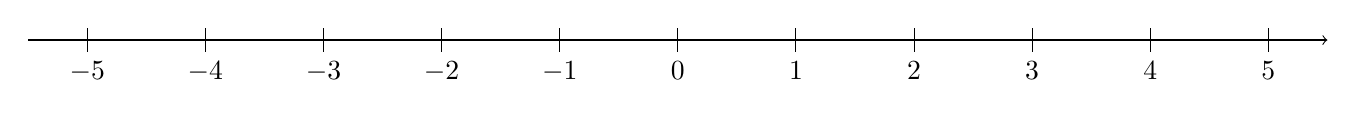
\begin{tikzpicture}[scale=1.5]
    \draw[->] (-5.5,0)--(5.5,0);
    \foreach \x in {-5,..., 4}{
        \draw (\x,0.1)--(\x,-0.1) node[below] {\(\x\)};
    }
        \draw (5,0.1)--(5,-0.1) node[below] {\(5\)};
    \end{tikzpicture}

    \begin{enumerate}
        \item Placer les points A d'abscisse \(-3\) ; B d'abscisse \(1,6\) ; C d'abscisse \(3,4\) et D d'abscisse \(\dfrac{14}{3}\).
        \item Calculer les distances AB, BC, et DA.
    \end{enumerate}

    \begin{indication}
        Pour chaque distance, commence par repérer lequel des deux nombres est le plus grand, puis calcule (le plus grand) \(-\) (le plus petit). Par exemple, pour AB : \(1,6 > -3\), donc \(\text{AB} = 1,6-(-3)\).
    \end{indication}

    \begin{enumerate}
        \setcounter{enumi}{2}
        \item Que se passe-t-il si tu calcules (le plus petit) \(-\) (le plus grand) au lieu de (le plus grand) \(-\) (le plus petit) ? Compare les deux résultats obtenus pour une même distance.
    \end{enumerate}
\end{exo}

\begin{prop}
    La distance entre deux nombres \(a\) et \(b\) est égale à \(b-a\) si \(b\geq a\), ou à \(a-b\) si \(a\geq b\). Autrement dit, on prend toujours (le plus grand nombre) moins (le plus petit).

    Cette distance se note aussi \(|b-a|\) (on lit \og valeur absolue de \(b-a\) \fg{}). On a donc \(|b-a| = |a-b|\) : calculer dans un sens ou dans l'autre donne le même résultat.
\end{prop}

\section{Valeur absolue d'un nombre}

\begin{defi}
    La \textbf{valeur absolue} d'un nombre \(x\), notée \(|x|\), est la distance entre \(x\) et \(0\) sur une droite graduée.

    Ainsi : \(|x| = x\) si \(x\geq 0\), et \(|x| = -x\) si \(x<0\).
\end{defi}

\begin{exple}
    \(|5| = 5\) car \(5\geq 0\). \(\quad |-5| = -(-5) = 5\) car \(-5<0\).

    On remarque que \(|5| = |-5|\) : les nombres \(5\) et \(-5\) sont bien à la même distance de \(0\).
\end{exple}

\begin{exo}[][]
    Essayez d'enlever les valeurs absolues pour finir les calculs suivants :
    \begin{enumerate}
        \item \(|3-5| = \)
    \end{enumerate}

    \begin{indication}
        Traite d'abord ce qu'il y a \textbf{à l'intérieur} de la valeur absolue, comme s'il n'y avait pas de barres : \(3-5=-2\). Applique ensuite la définition à ce résultat : \(|-2| = 2\) car \(-2<0\).
    \end{indication}

    \begin{tasks}(3)
        \task[2.] \(|5-3| = \)
        \task[3.] \(|-6| = \)
        \task[4.] \(|34| = \)
        \task[5.] \(-|5| = \)
        \task[6.] \(|3|-|5| = \)
    \end{tasks}

    \begin{indication}
        Attention aux questions 5 et 6 : dans \(-|5|\), le signe \og \(-\) \fg{} est \textbf{devant} la valeur absolue, il ne fait pas partie de ce qu'il y a dans les barres. Calcule d'abord \(|5|\), puis applique le signe \(-\) au résultat. De même dans \(|3|-|5|\), calcule séparément \(|3|\) et \(|5|\) avant de soustraire.
    \end{indication}
\end{exo}

\section{Résoudre une inéquation avec une valeur absolue}

\begin{met}
    Pour résoudre une inéquation du type \(|x-a| < r\) (avec \(r>0\)) :
    \begin{enumerate}
        \item traduire l'inéquation en langage de distance : \og la distance entre \(x\) et \(a\) est strictement inférieure à \(r\) \fg{} ;
        \item faire un schéma sur une droite graduée : placer \(a\), puis reculer de \(r\) et avancer de \(r\) ;
        \item lire les deux bornes de l'intervalle obtenu ;
        \item écrire l'ensemble des solutions sous forme d'intervalle.
    \end{enumerate}
\end{met}

\begin{exple}
    Résolvons \(|x-3|<5\). Cela signifie que la distance entre \(x\) et \(3\) est strictement inférieure à \(5\) : \(x\) doit donc se trouver entre \(3-5=-2\) et \(3+5=8\).

    \vspace{0.3cm}
    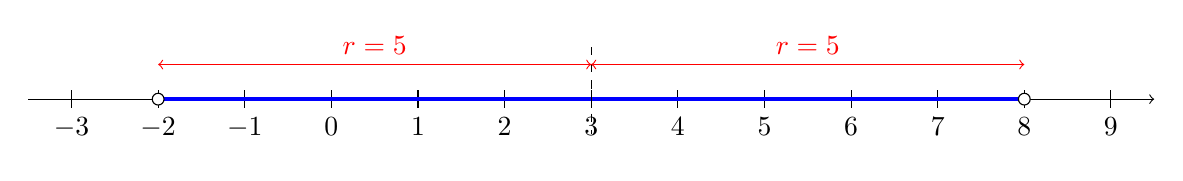
\begin{tikzpicture}[scale=1.1]
        \draw[->] (-3.5,0)--(9.5,0);
        \foreach \x in {-3,...,9}{
            \draw (\x,0.1)--(\x,-0.1) node[below] {\(\x\)};
        }
        \draw[very thick, blue] (-2,0)--(8,0);
        \draw[dashed] (3,0.6)--(3,-0.4) node[below] {};
        \draw[<->, red] (3,0.4)--(8,0.4) node[midway, above] {\(r=5\)};
        \draw[<->, red] (-2,0.4)--(3,0.4) node[midway, above] {\(r=5\)};
        \node[circle, draw, fill=white, inner sep=1.5pt] at (-2,0) {};
        \node[circle, draw, fill=white, inner sep=1.5pt] at (8,0) {};
    \end{tikzpicture}

    Les bornes \(-2\) et \(8\) ne sont pas solutions (l'inégalité est stricte), donc l'ensemble des solutions est l'intervalle \(]-2\ ;\ 8[\).
\end{exple}

\begin{exo}[][]
    Écrire sous la forme d'un intervalle l'ensemble des nombres \(x\) tels que :
    \begin{tasks}(2)
        \task \(|x-11|\leq 2\)
        \task \(|x+12|<2\)
    \end{tasks}

    \begin{indication}
        Pour \(|x-11|\leq 2\), attention à l'inégalité \textbf{large} : les deux bornes font cette fois partie des solutions (crochets fermés).

        Pour \(|x+12|<2\), remarque que \(|x+12| = |x-(-12)|\) : il s'agit donc de la distance entre \(x\) et \(-12\), et on peut appliquer la même méthode qu'avec \(|x-3|<5\), en remplaçant \(3\) par \(-12\).
    \end{indication}
\end{exo}

\begin{rem}
    Le symbole \(\cup\) se lit \og union \fg{} : \(A\cup B\) désigne l'ensemble des nombres qui appartiennent à \(A\) \textbf{ou} à \(B\) (éventuellement aux deux). On l'utilise quand l'ensemble des solutions est formé de plusieurs morceaux séparés.
\end{rem}

\begin{exo}[][appro]
    On souhaite résoudre \(|x|\geq 4\).
    \begin{enumerate}
        \item Traduire cette inéquation en langage de distance (par rapport à quel nombre ?).
        \item Sur une droite graduée, colorier tous les nombres qui conviennent. Obtiens-tu un seul morceau, ou plusieurs ?
        \item En déduire l'ensemble des solutions de \(|x|\geq 4\), écrit à l'aide d'un \(\cup\).
    \end{enumerate}

    \begin{indication}
        Contrairement à l'exemple \(|x-3|<5\), ici on cherche les nombres \textbf{loin} de \(0\) (à une distance d'\textbf{au moins} 4), et non les nombres proches de \(0\). Il y a donc les grands nombres positifs \textbf{et} les grands nombres négatifs (en valeur absolue) : deux morceaux, de part et d'autre de \(0\).
    \end{indication}
\end{exo}

\section{Vrai ou faux : propriétés de la valeur absolue}

\begin{indication}
    Pour montrer qu'une propriété est \textbf{fausse}, un seul \textbf{contre-exemple} (un exemple de nombres pour lesquels ça ne marche pas) suffit. Pour montrer qu'une propriété est \textbf{vraie pour tous les nombres}, un seul exemple ne suffit jamais : il faut utiliser la définition de la valeur absolue (vue en partie 2), et ce quels que soient les signes des nombres choisis.
\end{indication}

\begin{exo}[Vrai ou Faux][appro]

    Les propriétés suivantes sont-elles vraies ou fausses ? Justifier votre réponse.
    \begin{enumerate}
        \item Pour tous nombres \(a\) et \(b\), \(|a+b| = |a|+|b|\).
    \end{enumerate}

    \begin{indication}
        Essaie avec \(a=3\) et \(b=-3\) : calcule séparément \(|a+b|\) et \(|a|+|b|\), et compare.
    \end{indication}

    \begin{enumerate}
        \setcounter{enumi}{1}
        \item Il existe des nombres \(a\) et \(b\) tels que \(|a+b| = |a|+|b|\).
        \item Pour tout nombre réel \(a\), \(|-a|=|a|\).
    \end{enumerate}

    \begin{indication}
        Pour la question 2, il suffit de trouver \textbf{un} exemple qui fonctionne (par exemple avec deux nombres de même signe, ou l'un des deux nul).

        Pour la question 3, reviens à la définition de la partie 2 en distinguant les cas \(a\geq 0\) et \(a<0\), ou pense en termes de distance à \(0\).
    \end{indication}
\end{exo}

\begin{cbox}
\textbf{Bilan : as-tu compris cette partie ?} Coche ce que tu es capable de faire sans regarder la fiche.
\begin{itemize}
    \item[$\square$] Je sais expliquer avec mes mots ce qu'est la distance entre deux nombres.
    \item[$\square$] Je connais la définition de \(|x|\) et je sais l'appliquer à un nombre positif ou négatif.
    \item[$\square$] Je sais calculer une valeur absolue, y compris quand le signe \(-\) est \textbf{devant} les barres.
    \item[$\square$] Je sais résoudre \(|x-a|<r\) ou \(|x-a|\leq r\) en faisant un schéma.
    \item[$\square$] Je sais que \(|x|\geq r\) donne \textbf{deux} morceaux de solutions, reliés par \(\cup\).
\end{itemize}
Si tu as un \(\square\) que tu n'arrives pas à cocher, relis l'encadré correspondant avant de passer à la suite du chapitre.
\end{cbox}

\newpage
\section*{Corrigé}
\begin{indication}[À ne consulter qu'après avoir cherché !]
    Seuls les résultats finaux sont donnés ici : ils servent à vérifier ton travail, pas à le remplacer.
\end{indication}

\begin{enumerate}
    \item \textbf{Exercice 1.} Marie Curie : \(67\) ans. Aristote : \(-384\) et \(-322\), donc \(62\) ans. Qumran : \(218\) ans. Pythagore : né en \(560\) av. J.-C.
    \item \textbf{Exercice 2.} \(\text{AB}=4,6\) ; \(\text{BC}=1,8\) ; \(\text{DA}=\dfrac{23}{3}\) (soit environ \(7,67\)). Les deux ordres de soustraction donnent des résultats opposés (l'un est l'opposé de l'autre) ; la distance est la valeur \textbf{positive} des deux.
    \item \textbf{Exercice 3.} \(|3-5|=2\) ; \(|5-3|=2\) ; \(|-6|=6\) ; \(|34|=34\) ; \(-|5|=-5\) ; \(|3|-|5|=-2\).
    \item \textbf{Exercice 4.} \(|x-11|\leq 2 \iff x\in[9\ ;\ 13]\). \quad \(|x+12|<2 \iff x\in\ ]-14\ ;\ -10[\).
    \item \textbf{Exercice 5.} \(|x|\geq 4 \iff x\in\ ]-\infty\ ;\ -4]\cup[4\ ;\ +\infty[\).
    \item \textbf{Exercice 6.} 1. Faux (par exemple \(a=3\), \(b=-3\) : \(|a+b|=0\) mais \(|a|+|b|=6\)). 2. Vrai (par exemple \(a=3\), \(b=5\), ou dès que \(a\) et \(b\) sont de même signe, ou que l'un des deux est nul). 3. Vrai, pour tout réel \(a\).
\end{enumerate}

\end{document}
